\documentclass[12pt,a4paper]{article}

\usepackage[T1]{fontenc}
\usepackage[utf8]{inputenc}
\usepackage[english]{babel}
\usepackage{microtype}
\usepackage{amsmath,amsfonts,amssymb,amsthm,mathtools}
\usepackage{graphicx}
\usepackage{url}
\usepackage{geometry}
\usepackage{hyperref}
\usepackage{fancyhdr}
\usepackage{enumitem}
\usepackage{tabularx}
\usepackage{csquotes}
\usepackage{listings}

\geometry{left=3cm,right=3cm,top=3cm,bottom=3cm,headheight=15pt}

\hypersetup{
  colorlinks=true,
  linkcolor=blue,
  citecolor=blue,
  urlcolor=blue
}

\pagestyle{fancy}
\fancyhf{}
\fancyhead[L]{MATH 477 Applied Finite Element Analysis}
\fancyhead[R]{Homework Report}
\fancyfoot[C]{\thepage}
\renewcommand{\headrulewidth}{0.4pt}
\renewcommand{\footrulewidth}{0.4pt}

\newtheorem{theorem}{Theorem}
\newtheorem{lemma}{Lemma}

\lstset{
  language=Matlab,
  basicstyle=\ttfamily\small,
  numbers=left,
  numbersep=8pt,
  frame=single,
  breaklines=true,
  columns=fullflexible
}

\newif\ifhavebib
\IfFileExists{ref.bib}{\havebibtrue}{\havebibfalse}
\usepackage[style=apa]{biblatex}
\ifhavebib
  \addbibresource{ref.bib}
\fi

\graphicspath{{figs/}}

\begin{document}

\begin{titlepage}
  \centering

  {\Large\bfseries MATH 477 Applied Finite Element Analysis\par}
  \vspace{12pt}
  {\large Homework Report\par}
  \vspace{12pt}
  {\large \today\par}
  \vspace{12pt}

  % place a logo file into the project root or figs to show it
  \IfFileExists{figs/nu_logo.png}{\includegraphics[width=.25\textwidth]{figs/nu_logo.png}\par\vspace{8pt}}{}

  \vfill

  \begin{tabularx}{\textwidth}{@{}lX@{}}
    Student Name: & \textbf{Your Name} \\
    Student ID:   & \textbf{Your ID} \\
    Course:       & MATH 477 Applied Finite Element Analysis \\
    Instructor:   & Dongming Wei \\
    Subject Area: & Applied Finite Element Analysis \\
    Description:  & Homework solutions prepared in \LaTeX
  \end{tabularx}

  \vfill
  {\footnotesize By submitting this work I confirm that I have read the academic integrity policy and that all work is my own except where clearly cited.\par}
\end{titlepage}

\tableofcontents
\newpage

\section{Instructions summary}
Solve each boundary value problem by Laplace transform. Provide the exact solution \(u(x)\). Include a short check of boundary conditions and units. Plot \(u(x)\) in Matlab. Place Matlab listings in the appendix and export figures into the \texttt{figs} folder to include them in the report.

\section{Problem one}
\subsection{Statement}
Write the problem exactly as assigned.

\subsection{Solution by Laplace transform}
Show the steps for the transform in \(x\) as covered in class. State any transform identities you use. Derive \(U(s)\) and invert to obtain \(u(x)\). Simplify the expression.

\subsection{Checks}
\begin{itemize}[leftmargin=1.5em]
  \item Verify both boundary conditions.
  \item State the regularity of \(u\).
  \item Comment on physical interpretation if a distributed load \(g(x)\) is present.
\end{itemize}

\subsection{Plot}
Include the Matlab figure.
\begin{figure}[h]
  \centering
  \IfFileExists{figs/p1_u.png}{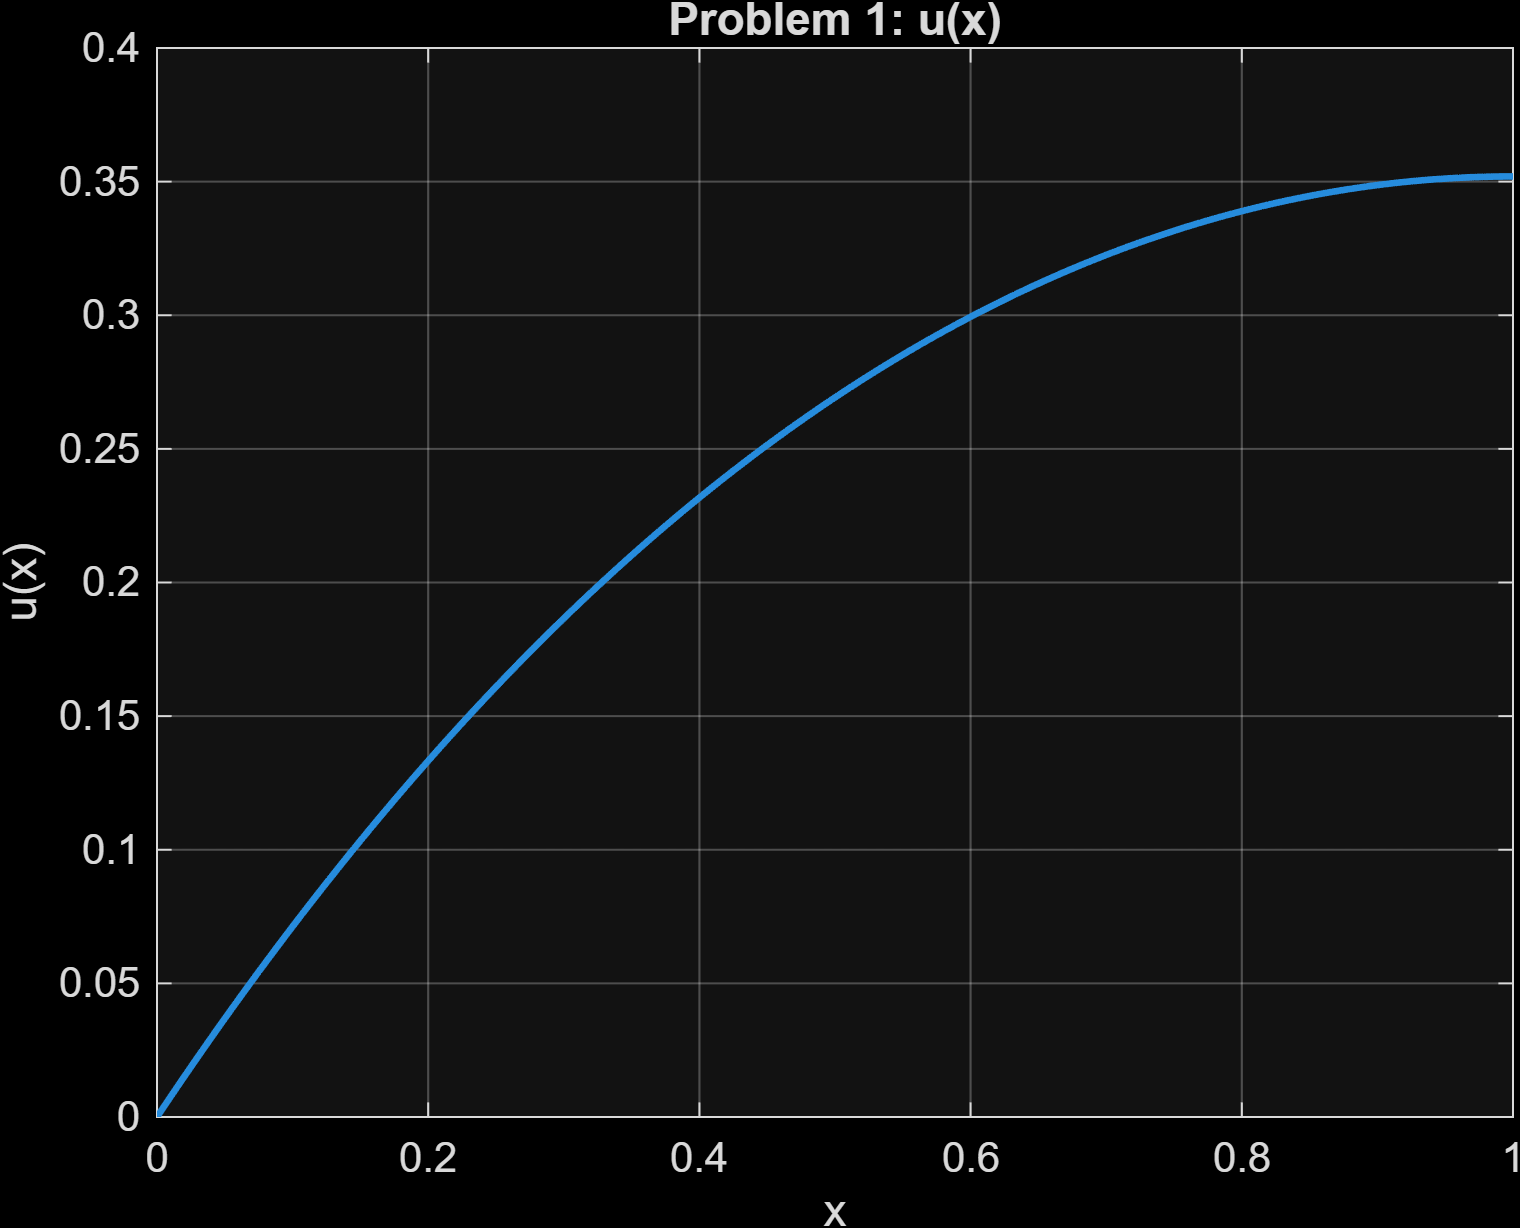
\includegraphics[width=.7\linewidth]{figs/p1_u.png}}{\fbox{\rule{0pt}{3cm}\rule{.7\linewidth}{0pt}}}
  \caption{Graph of \(u(x)\) for Problem one}
\end{figure}

\section{Problem two with a point source}
\subsection{Statement}
Write the problem with Dirac delta at \(x=x_{0}\).

\subsection{Solution by Laplace transform}
Work out the transform and inversion. Describe the jump in \(u'(x)\) at \(x_{0}\) and how it arises from the delta source.

\subsection{Checks}
\begin{itemize}[leftmargin=1.5em]
  \item Verify boundary conditions.
  \item Verify the jump condition for \(u'(x)\) at \(x_{0}\).
\end{itemize}

\subsection{Plot}
\begin{figure}[h]
  \centering
  \IfFileExists{figs/p2_u.png}{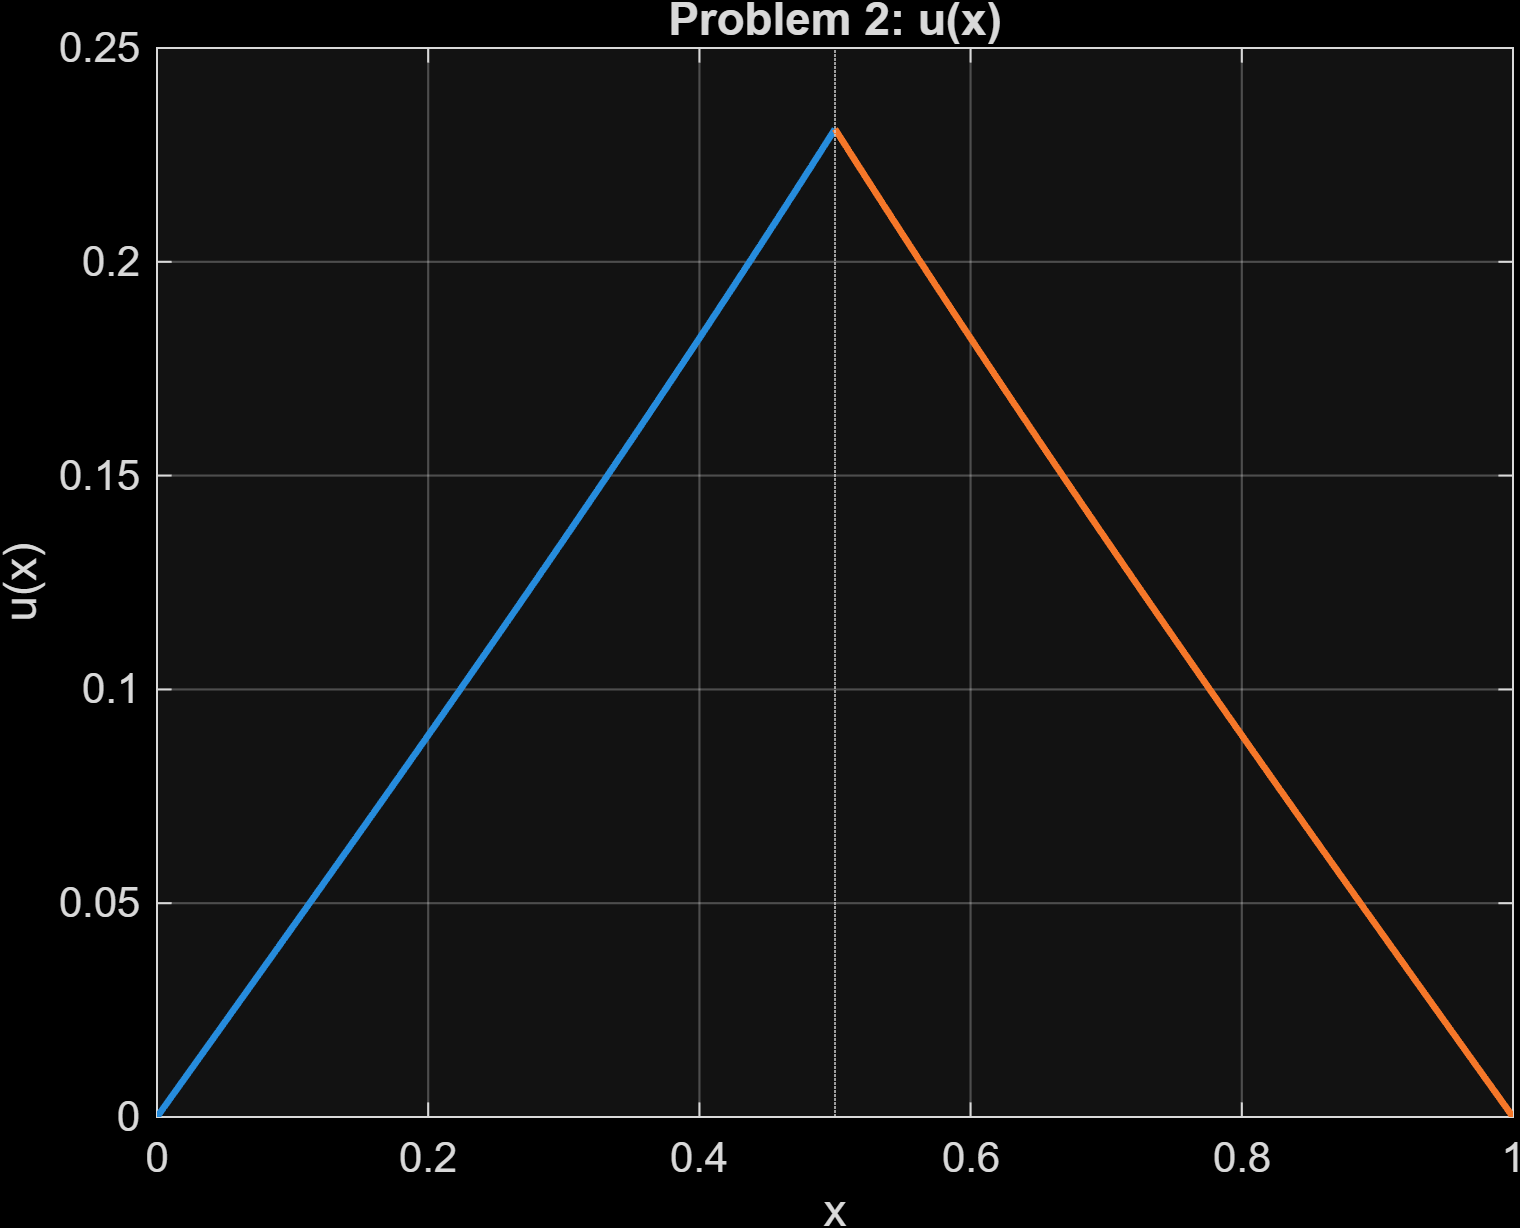
\includegraphics[width=.7\linewidth]{figs/p2_u.png}}{\fbox{\rule{0pt}{3cm}\rule{.7\linewidth}{0pt}}}
  \caption{Graph of \(u(x)\) for Problem two}
\end{figure}

\section{Problem three}
\subsection{Statement}
Write the third problem exactly as assigned.

\subsection{Solution by Laplace transform}
Provide full derivation and the final closed form of \(u(x)\).

\subsection{Checks}
Confirm boundary conditions and discuss limiting cases.

\subsection{Plot}
\begin{figure}[h]
  \centering
  \IfFileExists{figs/p3_u.png}{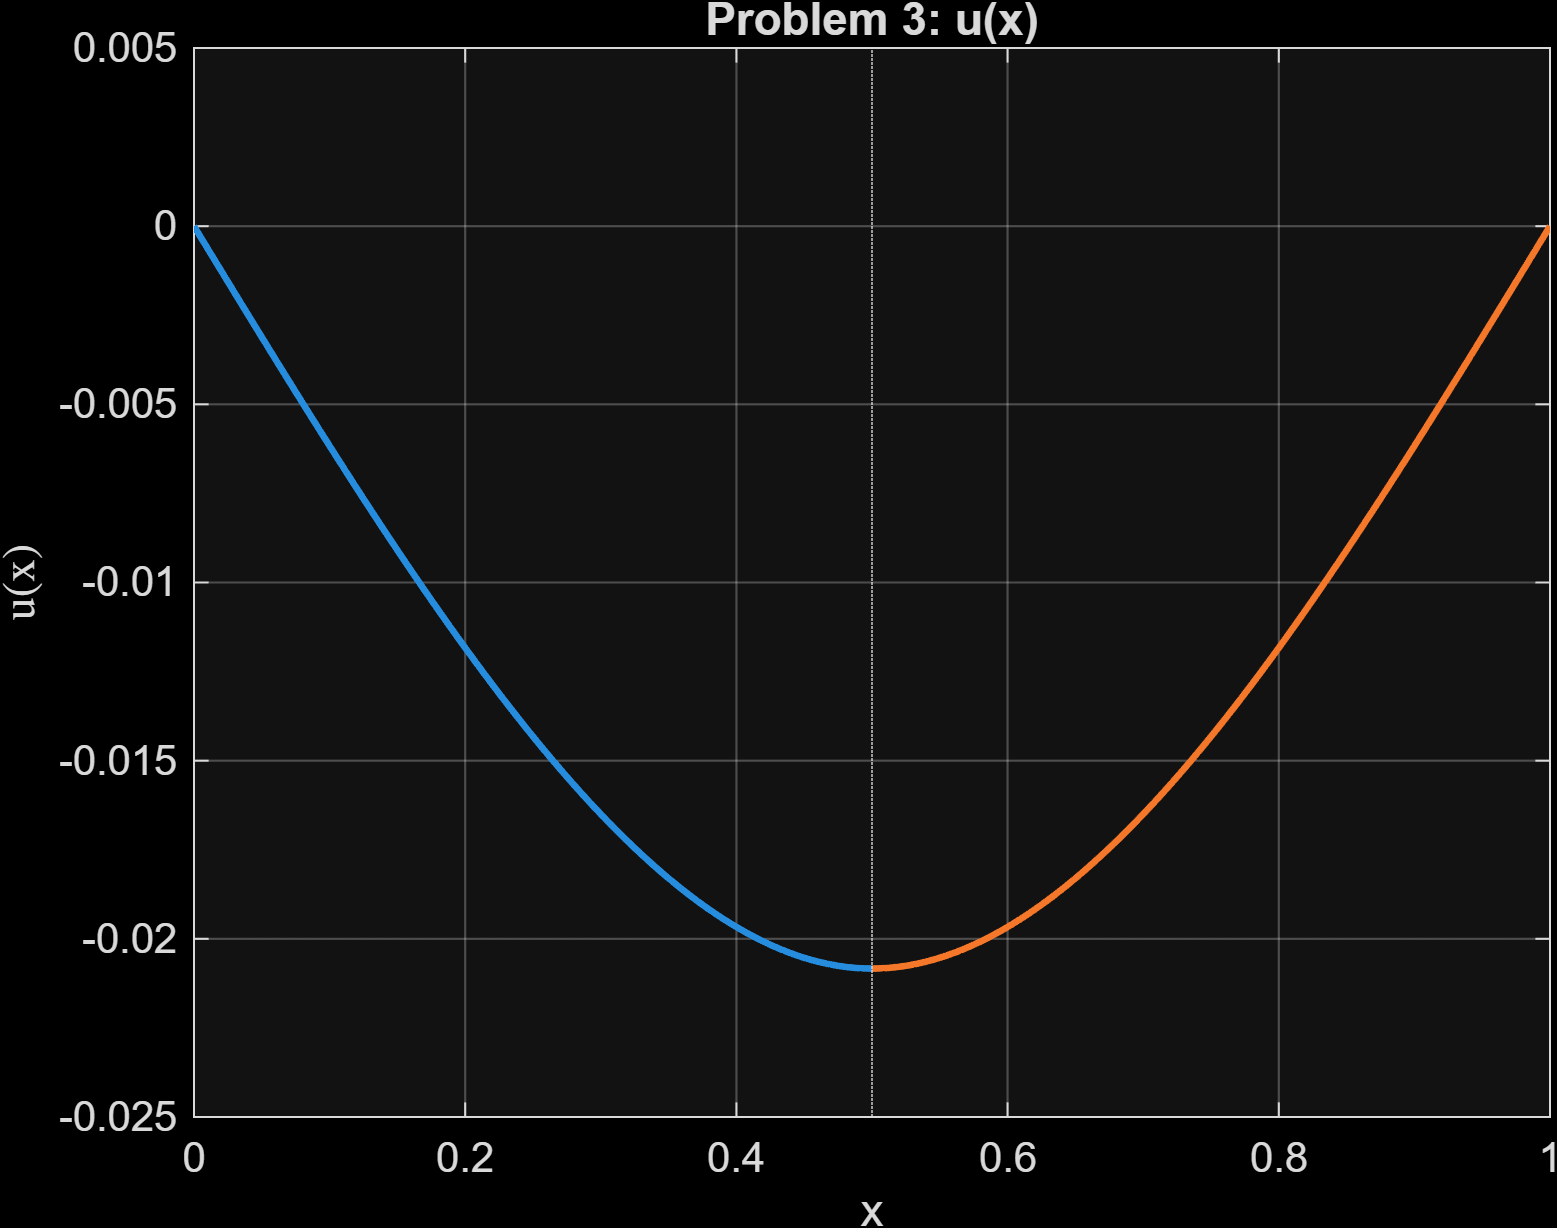
\includegraphics[width=.7\linewidth]{figs/p3_u.png}}{\fbox{\rule{0pt}{3cm}\rule{.7\linewidth}{0pt}}}
  \caption{Graph of \(u(x)\) for Problem three}
\end{figure}

\section{Conclusion}
Summarize the method and any observations from the plots.

\ifhavebib
\newpage
\printbibliography
\fi

\appendix
\section{Matlab code}
Place clean Matlab scripts here.

\subsection*{Problem one script}
\begin{lstlisting}
% p1_plot.m
% create x grid
x = linspace(0,1,400);
% example placeholder solution shape
u = x .* (1 - x);
plot(x,u,'LineWidth',1.5);
xlabel('x'); ylabel('u(x)');
title('Problem one');
saveas(gcf,'figs/p1_u.png');
\end{lstlisting}

\subsection*{Problem two script}
\begin{lstlisting}
% p2_plot.m
x0 = 0.4;
x  = linspace(0,1,400);
% toy profile with a kink at x0
u = x .* (1 - x);
u(x >= x0) = u(x >= x0) + 0.1*(x(x >= x0) - x0);
plot(x,u,'LineWidth',1.5);
xlabel('x'); ylabel('u(x)');
title('Problem two');
saveas(gcf,'figs/p2_u.png');
\end{lstlisting}

\subsection*{Problem three script}
\begin{lstlisting}
% p3_plot.m
x = linspace(0,1,400);
u = sin(pi*x);
plot(x,u,'LineWidth',1.5);
xlabel('x'); ylabel('u(x)');
title('Problem three');
saveas(gcf,'figs/p3_u.png');
\end{lstlisting}

\end{document}
